\documentclass[12pt,a4paper]{report}
\usepackage[utf8]{inputenc}
\usepackage{graphicx}
\usepackage{amsthm,amsfonts,amssymb}
\usepackage{amsmath}
\usepackage[inline,shortlabels]{enumitem}
\usepackage{a4wide}
\usepackage{titlesec}
\usepackage{makeidx}
\usepackage{tikz-cd}
\usepackage{tikz}
\usepackage{braket}
\usepackage{zref}


\usetikzlibrary{matrix, calc, arrows, fit}
\tikzset{commutative diagrams/.cd}
\tikzset{commutative diagrams/row    sep/normal=1.3cm}
\tikzset{commutative diagrams/column sep/normal=1.3cm}
\makeindex

% Formating of theorems, lemmas, ...
\titlelabel{\thetitle.\quad}

\def\afterDotSpace{.5em}

% Proper labeling and referencing
% http://tex.stackexchange.com/questions/57799/refer-to-theorems-in-previous-chapter
\makeatletter
\let\oldlabel\label
\renewcommand{\label}[1]{%
  \zref@labelbylist{#1}{special}% Special label
  \oldlabel{#1}% Old label
}
\newcounter{splabel}
\zref@newlist{special}% Create a new property list called special
\zref@newprop{chapter}{\Roman{chapter}}% Section property holds \arabic{chapter}
\zref@addprop{special}{chapter}% Add a chapter property to special
\let\oldref\ref
\newcommand*{\thmref}[1]{%
  \stepcounter{splabel}% Increment local "special label" counter
  \zref@labelbylist{#1-\thesplabel}{special}% Create label
  \edef\targetchap{\zref@extractdefault{#1}{chapter}{-1}}% Extract target chapter
  \edef\sourcechap{\zref@extractdefault{#1-\thesplabel}{chapter}{-1}}% Extract source chapter
  % (My modification) The way how to compare two strings:
  \ifnum\pdfstrcmp{\targetchap}{\sourcechap}=0\else\targetchap.\fi%
  \oldref{#1}%
}
\renewcommand\ref[1]{\thmref{#1}}
\makeatother

% Counting and environments
\newcounter{thmCounter}[section]
\renewcommand \thechapter{\Roman{chapter}}
\renewcommand \thesection{\arabic{section}}
\renewcommand{\thethmCounter}{\thesection.\arabic{thmCounter}}

\def\blockHelperA{\par\medskip\noindent}
\def\blockHelperB{\refstepcounter{thmCounter}\textbf{\arabic{section}.\arabic{thmCounter}.}}
\def\blockHelperCA{\hspace{\afterDotSpace}\ignorespaces}
\def\blockHelperCB{\it\blockHelperCA}

\def\blockEnv#1{\blockHelperA\blockHelperB{\bf~#1.}\blockHelperCA}
\def\blockEnvS#1{\blockHelperA{\bf #1.}\blockHelperCA}
\def\blockPropEnv#1{\blockHelperA\blockHelperB{\bf~#1.}\blockHelperCB}
\def\blockPropEnvS#1{\blockHelperA{\bf #1.}\blockHelperCB}
\def\endBlockEnv{\par\medskip}

% TODO add little space before numbered paragraph
\def\num{\blockHelperA\blockHelperB\hspace{\afterDotSpace}}

\newenvironment{block}{\blockEnv}{\endBlockEnv}
\newenvironment{block*}{\blockEnvS}{\endBlockEnv}
\newenvironment{blockProp}{\blockPropEnv}{\endBlockEnv}
\newenvironment{blockProp*}{\blockPropEnvS}{\endBlockEnv}

\newtheoremstyle{newthmstyle}% name of the style to be used
    {8pt}% measure of space to leave above the theorem. E.g.: 3pt
    {3pt}% measure of space to leave below the theorem. E.g.: 3pt
    {\itshape}% name of font to use in the body of the theorem
    {}% measure of space to indent
    {\bfseries}% name of head font
    {.}% punctuation between head and body
    {\afterDotSpace}% space after theorem head; " " = normal interword space
    {\thmnumber{#2. }\thmname{#1}\thmnote{ \rm [#3]}}% Manually specify head

\newtheoremstyle{newthmstyleNormal}{8pt}{3pt}{}{}{\bfseries}{.}{\afterDotSpace}
    {\thmnumber{#2. }\thmname{#1}\thmnote{ \rm [#3]}}

\theoremstyle{newthmstyle}
\newtheorem{lemma}[thmCounter]{Lemma}
\newtheorem{theorem}[thmCounter]{Theorem}
\newtheorem{conclusion}[thmCounter]{Conclusion}
\newtheorem{proposition}[thmCounter]{Proposition}
\newtheorem{observation}[thmCounter]{Observation}
\newtheorem*{lemma*}{Lemma}
\newtheorem*{theorem*}{Theorem}
\newtheorem*{conclusion*}{Conclusion}
\newtheorem*{proposition*}{Proposition}
\newtheorem*{observation*}{Observation}

\theoremstyle{newthmstyleNormal}
\newtheorem{definition}[thmCounter]{Definition}
\newtheorem*{definition*}{Definition}

% Categories
\newcommand\categoryStyle[1]{\ensuremath{\mathbf{#1}}}
\newcommand\Frm{\categoryStyle{Frm}}
\newcommand\StoneFrm{\categoryStyle{StoneFrm}}
\newcommand\ExtrStoneFrm{\categoryStyle{ExtrDStoneFrm}}
\newcommand\Top{\categoryStyle{Top}}
\newcommand\StoneSp{\categoryStyle{StoneSp}}
\newcommand\Bool{\categoryStyle{Bool}}
\newcommand\ComplBool{\categoryStyle{ComplBool}}
\newcommand\CRegFrm{\categoryStyle{CRegFrm}}
\newcommand\RegKFrm{\categoryStyle{RegKFrm}}

% Special symbols
\newcommand\R{\ensuremath{\mathfrak{R}}}
\newcommand\C{\ensuremath{\mathcal{R}}}
\newcommand\J{\ensuremath{\mathfrak{J}}}
\newcommand\p[1]{\ensuremath{\mathcal{ #1 }}}
\newcommand\Bo{\ensuremath{\mathfrak{B}}} % booleanization
\newcommand\Bc{\ensuremath{\mathbb{B}}} % boolean/complemented elements
\newcommand\Sp{\ensuremath{\mathcal{S}}}
\newcommand\closure[1]{\overline{#1}}
\newcommand\upset  {\mathord{\uparrow}\mkern1mu}
\newcommand\downset{\mathord{\downarrow}\mkern1mu} % mathord/mathbin/mathrel treats symbol as oordinal math symbol/binary relation/...
\newcommand\rbelow{\prec}
\newcommand\crbelow{\rbelow\mkern-7mu\rbelow}
\DeclareMathOperator{\id}{id}
\DeclareMathOperator{\Id}{Id}
\DeclareMathOperator{\Ult}{Ult}
\def\InclUp{\rotatebox[origin=c]{90}{$\subseteq$}}
\def\DotsUp{\rotatebox[origin=c]{90}{\dots}}

% Function restriction
% http://tex.stackexchange.com/questions/22252/how-to-typeset-function-restrictions
\newcommand\restr[2]{{% we make the whole thing an ordinary symbol
  \left.\kern-\nulldelimiterspace % automatically resize the bar with \right
  #1 % the function
  \vphantom{\big|} % pretend it's a little taller at normal size
  \right|_{#2} % this is the delimiter
}}

% Other stuff
\newcommand\DEF[2][]{\emph{#2}\index{#2#1}}
  % example \DEF[|see{null-dimensional}]{zero-dimensional}
\newcommand\DEFSYM[3][a ]{\emph{#3}\index{#1#2@#3}\ignorespaces}

\newenvironment{diagram}{\begin{center}\begin{tikzcd}}{\end{tikzcd}\end{center}}
\newcommand\ACP{\hfill\fontshape{n}{\textbf{($\star$)}}}

\title{Some point--free aspects of connectedness}
\author{Tom\'a\v s Jakl}

\begin{document}
\maketitle
\tableofcontents

\chapter{Introduction}

In 1936 Marshall Stone made a great breakthrough in algebra and topology by publishing a paper called ``The Theory of Representations of Boolean Algebras''~\cite{stone1936theory}.
In this paper he described structural similarities between Boolean algebras and a certain class of topological spaces.
Besides that, he was also the first who constructed an example of a space which did not have the origin in geometry (as a subset of Euclidean space) and was constructed from an algebraic structure~\cite{johnstone1986stone}.

% The Stone representation theorem, or in other words the Stone duality, had a great impact in topology, functional analysis or representation theory of rings~\cite{johnstone1986stone}.
% TODO introduce Stone duality and Stone type dualities -- as an important example of a Stone type duality is Hofmann--Lawson's duality/... between .../spatial frames and sober? topological spaces

Frames and locales in point--free topology are natural generalizations of the notion of topological space.
These generalized spaces come out from an algebraical description of properties of the open set lattice.
Results from point--free topology often brings a new insight to classical results from general topology.
In contrast to general (set--theoretical) topology, a large part of the theory of frames and locales is given constructively.
This phenomenon is nicely expressed by the famous slogan of Banaschewski~\cite{banaschewski1990proving}:
\begin{center}\em
    Choice--free localic argument + suitable choice principle = classical result in spaces.
\end{center}


In this thesis, we present the Stone representation theorem, or later known as Stone duality, in point--free contex.
% In our case, it is a correspondence between Boolean algebras and Stone frames.
The slogan of Banaschewski has been fulfilled again even though we present the theorem in the language of frames instead of locales.
With Boolean Ultrafilter Theorem, we obtain the classical Stone duality for topological spaces.
It is not a surprise that the Stone duality in point--free setting happened to be a lot simpler than the original.
We do not have to be concerned about points.
% We work only with purely algebraic structures.

The point--free approach allow us to easily analyse particular parts of Stone duality.
For each infinite regular cardinal $\kappa$, we show that the counterpart to the $\kappa$--complete Boolean algebras on the frame side are the $\kappa$--basically disconnected Stone frames.
We also give a precise characterisation of the morphisms which correspond to the $\kappa$--complete Boolean homomorphisms.

Booleanization is the construction of Boolean algebra from Heyting algebra by taking the set of elements of the form $a = a^{**}$.
For a topological space, Booleanization of its frame of open sets is the set of all regular open subsets and it forms a complete Boolean algebra.
In point--free topology, one has an another useful property.
Booleanization of a locale is the smallest dense sublocale of that locale~\cite{banaschewski1996booleanization}.

Analogously to Stone duality for topological spaces, the frames corresponding to the complete Boolean algebras are precisely the extremally disconnected Stone frames.
Hence, we have a proper class of variants of disconnectedness in between zero--dimensionality and extremal disconnectedness. % TODO
Interestingly, Booleanization is functorial for this part of duality and it is an isomorphism of the complete parts of the duality.

At the end of the thesis we focus on De Morgan (or extremally disconnected) frames.
We show a new characterisation of completely regular De Morgan frames.
A completely regular frame is De Morgan if and only if each dense sublocale of the frame is superdense.
Counter to that are the compact metric frames, they have no non-trivial superdense sublocale.
Consequently, a non-trivial \v{C}ech--Stone compactification of metrizabile frame is never metrizabile.

% TODO Consider:  So compact regular frm is de morgan <=> compactification of Booleanization is the original frame?

\subsection*{Organization of the thesis}

In Chapter II we present necessary facts from order theory, category theory and topology which we will need in the subsequent chapters.
In Chapter III are discussed several disconnected properties and \v{C}ech--Stone compactification. % TODO
In Chapter IV we present the Stone duality in both point--free and set--theoretical setting.
Chapter V is devoted to particular parts of Stone duality.
In Chapter VI we show that Booleanization is an isomorphisms of the complete parts of Stone duality.
Finally, in Chapter VII we present a new characterisation of De Morgan frames and non--metrizability of non--trivial \v{C}ech--Stone compactification.

% Chapters II and III consist of well--known facts and I am not an author of any of them.
The theorems in the last chapter as well as the idea to take a look at Booleanization are due to Professor Pultr.

We assume from the reader experiences with abstract algebra, topology and set theory.
A familiarity with the basic notions of category theory is an advantage but not necessity.

The propositions which rely on Axiom of Choice or Boolean Ultrafilter Theorem are marked by  \ACPStar{}.
The chapter numbers are omitted whenever we refer to the same chapter.

\chapter{Preliminaries}
We assume basic knowledge of Set Theory, mainly basic knowledge about cardinals and cardinalities, ``axiom of choice''.

We refer to the monograph \emph{Frames and Locales} written by Pultr and Picado~\cite{picado2011frames} as a basic introduction to point--free topology.

\section{Partially ordered set}

\num Let $A$ be a set and let $\leq$ be a binary relation on $A$ ($(\leq) \subseteq A\times A$). We say $(A, \leq)$ is a \DEF{partially ordered set} if the relation $\leq$ is \emph{partial order}, i.e. satisfies:
\begin{enumerate}[(P1)]
    \item \emph{reflexivity:} $a \leq a$ for all $a \in A$,
    \item \emph{antisymmetry:} $a \leq b$ and $b\leq a$ implies $a = b$ for all $a,b \in A$,
    \item \emph{transitivity:} $a \leq b$ and $b\leq c$ implies $a \leq c$ for all $a,b,c \in A$.
\end{enumerate}

Denote by $(A,\leq)^{\op}$ the partially ordered set $(A,\leq')$ such that $(\leq') = \Set{ (b,a) \in A\times A | a\leq b}$.

% TODO better wording
Let $S$ be a subset of $A$.
We say $u$ is an upper bound for $S$ if $u \geq x$ for all $x$ of $S$. We say $s$ is a supremum for $S$ if $s$ is the least upper bound for $S$. We write $s = \bigvee S$.
We say $l$ is an lover bound for $S$ if $l \leq x$ for all $x$ of $S$. We say $i$ is a infimum for $S$ if $i$ is the supremum for $S$ in $A^{\op}$, i.e. if $i$ is the greatest lower bound for $S$. We write $i = \bigwedge S$.

A partially ordered set $(A,\leq)$ is \emph{join semilattice} if each two element subset has a supremum. Similarly, \emph{meet semilattice} has an infimum for each two element subset.
A \DEF{lattice} is partially ordered set which is both join-- and meet-- semilattice. We write $a\vee b$ (\emph{meet}) for the supreum of $\{a,b\}$ and $a\wedge b$ (\emph{join}) for the infimum.

A mapping $f\colon A\to B$ between two partially ordered sets is called \emph{monotone} if $f(x)\leq f(y)$ wherever $x\leq y$. If, moreover, $A$ and $B$ are lattices and $f(x\vee y) = f(x)\vee f(y)$ and $f(x\wedge y) = f(x)\wedge f(y)$ for all $x,y\in A$, we say $f$ is a \emph{lattice homomorphism}.

\num A lattice is called a \DEF{complete lattice} if every subset has an infimum and a supremum.

\begin{theorem*}
    For a lattice $L$ are the following conditions equivalent:
    \begin{itemize}
        \item $L$ is a complete lattice;
        \item every subset of $L$ has a supremum;
        \item every subset of $L$ has an infimum.
    \end{itemize}
\end{theorem*}

For a complete lattice we therefore have two infinitary operations the meet $\bigvee$ and the join $\bigwedge$.
Note that every complete lattice contains two distinguished elements: 0 and 1, where $0 = \bigvee \emptyset$ and $1 = \bigwedge \emptyset$.

A lattice homomorphism $f\colon A\to B$ between two complete lattices is \DEF{complete lattice homomorphism} if $f(\bigvee X) = \bigvee f[X]$ and $f(\bigwedge X) = \bigwedge f[X]$ for each subset $X \subseteq A$.

\num A lattice $D$ is \DEF{distributive} if the following equation holds for all $a,b,c\in D$:
\begin{align}
    a\vee (b\wedge c) = (a\vee b)\wedge (a\vee c).\tag{Dist}
\end{align}

\begin{theorem*}
    For a lattice $D$, the following conditions are equivalent:
    \begin{itemize}
        \item $D$ is a distributive lattice,
        \item $a\vee (b\wedge c) = (a\vee b)\wedge (a\vee c)$ for all $a,b,c \in D$,
        \item For each $a,b,c\in D$ there exists at most one $x$ such that
            \begin{align*}
                a\vee x &= b\\
                a\wedge x &= c.
            \end{align*}
    \end{itemize}
\end{theorem*}

\num Let $A$ and $B$ be two partially ordered sets. Two monotone mappings $f\colon A \to B$ and $g\colon B\to A$ are in \DEF{Galois connection} or are \DEF{Galois adjoing} if
$$ f(x) \leq y\quad\text{iff}\quad x\leq g(y)\quad\text{for all } x\in A, y\in B.$$

\noindent Or equivalently
$$ fg(y) \leq y\quad\text{and}\quad x\leq gf(y)\quad\text{for all } x\in A, y\in B.$$

Then we say $f$ is a left Galois adjoing and a $g$ is a right Galois adjoing.
For a monotone map, its left or right Galois adjoint do not need to exists but if they do, they are uniquely determined.

Consequently, for two monotone maps in Galois connection $f,g$ we have that
$$ f g f = f\quad\text{and}\quad g f g = g. $$

\begin{theorem*}
    For a monotone map $f\colon A\to B$, if $f$ is a left (resp. right) Galois adjoint
    then $f$ preserves all existing suprema (resp. infima).

    Moreover, the converse implication also holds if $A$ and $B$ are complete lattices.
\end{theorem*}

\num Let $L$ be a lattice with 0. A pseudocomplement $a^*$ for an element $a\in L$ is the greatest element $x$ such that
$$ x\wedge a = 0. $$

\noindent Equivalently, $a^*$ is the pseudocomplement of $a$ if
$$ x\wedge a = 0 \quad\text{iff}\quad x\leq a^*\quad\text{for all } x\in L. $$

A lattice is called \DEF{pseudocomplemented}[ lattice] if every element has a pseudocomplement.

\begin{proposition*}\label{p:pseudcomplProperties} Properties of pseudocomplement.
\begin{enumerate}
    \item $a \leq a^{**}$, $a^* = a^{***}$,
    \item $a \leq b \implies a^* \geq b^*$,
    \item $(a \wedge b)^{**} = a^{**} \wedge b^{**}$.
\end{enumerate}
\end{proposition*}

\num Heyting algebras, $\_^* = \_ \to 0$
\num Boolean algebras and Boolean homomorphisms, \DEF{\Bool}
\num filters, ideals, principal filter/ideal, prime/maximal/ultrafilter on BA
\num Axiom of Choice/Zorn's Lemma, Boolean Ultrafilter Theorem

\section{Category Theory}
\begin{itemize}
    \item category (in basic definition locally small), demonstrative  examples using categories from previous section (most importantly \Bool), dual category??
    \item functor (important example: identity functor and constant functor), covariant, contravariant
    \item natural transformation, natural equivalence, functor category
    \item limits/colimits via "universal functors", example products, sums
    \item ajdunction only via units and counits of adjunction

    explain importance of adjunction by mentioning the limit preserving
\end{itemize}

\section{Topology and point--free Topology}

\num Basic definitions: topology, frame, their categories, functor $\Omega$, \Top{} and \Frm. frame homomorphisms, localic maps, continuous map, homeomorphism

\num Separation axioms (regularity, complete regularity, normality, ...?), rather below (and useful facts about them)

\num\label{p:rbellowProperties} $a_1\wedge a_2 \rbelow b_1 \wedge b_2$ and $a_1\vee a_2 \rbelow b_1 \vee b_2$ for $a_i\rbelow b_i$
\num\label{p:crbellowProperties} $a_1\wedge a_2 \crbelow b_1 \wedge b_2$ and $a_1\vee a_2 \crbelow b_1 \vee b_2$ for $a_i\crbelow b_i$
                                   $a \crbelow x\crbelow y\crbelow b$ implies $b^* \crbelow x\crbelow y\crbelow a^*$

    Again, as for topological spaces, we have:

    \num\label{p:normalRegular} Any normal and regular frame is completely regular: For $x\rbelow y$, the $x^*\vee y = 1$ holds, from normality there exists a $q$, such that $x^*\vee q = 1$ and $q^*\vee y = 1$, thus $x\rbelow q\rbelow y$. So $\Set{x | x\rbelow b} = \Set{x | x\crbelow b}$

    $T_4 + T_1 \implies T_{3.5} + T_0 \implies T_3 + T_0 \implies T_2 \implies T_1 \implies T_0$

\num completeness and cocompleteness of \Top{} and \Frm{}
\num Spatiality, some spatiality theorems (II.5.3, Hofmann--Lawson's Duality)
\num Subspace and sublocale/subframe, dense sublocale, empty frame (\emptyFrm), co-frame of sublocales (we will need its distributivity), $\iota_S\colon L \to S$ as subframe inclusion and as onto frame homomorphisms? (the next part needs it)

\begin{block*}{Note}
    We will call sublocales which are both open and closed as clopen. % TODO check grammar
\end{block*}

TODO place somewhere StoneSp and StoneFrm and \J.

Notation.
$\downset a^*$ means $\downset (a^*)$ (rightmost unary operator applies first)

For the definition of frames, we see that $\wedge$ is the left/right Galois adjoint, therefore every frame is a complete Heyting algebra, moreover also a pseudocomplemented lattice. The pseudocomplement operation for open set in spacial frames corresponds precisely to the complement of the closure of that set, or the interior of the complement.

\begin{definition}
    Let $L$ be a locale, \DEF{nucleus} $\nu$ on $L$ is a monotone map $\nu\colon L \to L$ having the following four properties:
    \begin{enumerate}[(N1)]
        \item $a \leq \nu(a)$,
        \item $a \leq b \implies \nu(a) \leq \nu(b)$,
        \item $\nu\nu(a) = \nu(a)$, and
        \item $\nu(a \wedge b) = \nu(a) \wedge \nu(b)$.
    \end{enumerate}
\end{definition}

\num\label{p:nuclProp} \textbf{Properties of nuclei.} For a locale $L$ and a nucleus $\nu\colon L \to L$, set $S = \nu(L)$. The set $S$ together with suprema and infima defined
    $$ \bigsqcup a_i = \nu(\bigvee a_i)\quad\text{ and }\quad a \sqcap b = a \wedge b$$

\noindent is a sublocale of $L$. Indeed, we have
$$ (\bigsqcup a_i)\sqcap b = \nu(\bigvee a_i) \wedge \nu(b) = \nu(\bigvee(a_i \wedge b)) = \bigsqcup (a_i \sqcap b).$$

\noindent From (N4) we know, $\sqcap$ is the infimum and from (N2) we know $\bigsqcup$ is the supremum. Hence $\nu(L)$ is a locale, to show that $\nu(L)$ is a sublocale of $L$ for $\nu^*\colon L \to \nu(L)$, defined $a \mapsto \nu(a)$, we will show it is an onto frame homomorphism. It is enough to show
    $$\nu(\bigvee a_i) = \nu(\bigvee \nu(a_i)) \quad( = \bigsqcup \nu(a_i)).$$

    \noindent We have $\bigvee a_i \leq \bigvee \nu(a_i)$ by (N1) and $\nu(\bigvee a_i) \leq \nu(\bigvee \nu(a_i))$ by (N2). On the other hand $\nu(a_i) \leq \nu(\bigvee a_i)$ by (N2). Hence $\bigvee \nu(a_i) \leq \nu(\bigvee a_i)$ and $\nu(\bigvee \nu(a_i)) \leq \nu\nu(\bigvee a_i) = \nu(\bigvee a_i)$ by (N2) and (N3).

\chapter{Connectedness and Compactification}

Compactness, connectedness and variants of disconnectedness are commonly studied properties of topological spaces. In this chapter, we will prove some results which are well known from Set theoretical topology and we will prove them in the context of point--free topology.

\section{Connectedness and variants of disconnectedness}
\begin{definition}
    We say a frame $L$ is \DEF{disconnected} if $L$ contains non-trivial elements $a$ and $b$ (that is, different from the top and the bottom of $L$) such that $a\vee b = 1$ and $a\wedge b = 0$. If a frame is not disconnected, we say it is \DEF{connected}.
\end{definition}

\begin{observation}\label{p:disconnectednessEquivalently}
    For a frame $L$, the following conditions are equivalent:

    \begin{enumerate}
        \item $L$ is disconnected.
        \item There exists a non-trivial both open and closed sublocale of $L$ (that is, different from $\emptyFrm$ and $L$).
        \item There exists an one-one frame homomorphism $f\colon $\DEFSYM{B2}{$B_2$}$ \to L$, where $B_2$ is the Boolean algebra on four elements.
    \end{enumerate}
\end{observation}

\begin{lemma}
    Let $L$ be a frame. The following are equivalent:

    \begin{enumerate}
        \item Closure of each open sublocale of $L$ is open.
        \item For all $a \in L$: $\closure{\mathfrak{o}(a)} = \mathfrak{o}(a^{**})$.
        \item For all $a \in L$: $a^{**} \vee a^* = 1$.
    \end{enumerate}
\end{lemma}
\begin{proof}
    The implication from 2.\ to 1.\ is trivial. For the implication from 3.\ to 2., first observe that
    \begin{align*}
        \open(a^{**})\vee \open(a^*) &= \open(a^{**}\vee a^*) = \open(1) = L, \text{ and} \\
        \open(a^{**})\wedge \open(a^*) &= \open(a^{**}\wedge a^*) = \open(0) = \emptyFrm.
    \end{align*}

    \noindent However, $\open(a^*)$ is complemented with $\clos(a^*)$. In other words
    \begin{align*}
        \clos(a^*)\vee \open(a^*) &= L, \text{ and} \\
        \clos(a^*)\wedge \open(a^*) &= \emptyFrm.
    \end{align*}

    \noindent By distributivity of the frame of all all sublocales of $L$, $\open(a^{**}) = \clos(a^*) = \closure{\open(a)}$.

    Finally, for the implication from 1.\ to 3.: $\closure{\open(a)} = \clos(a^*) = \open(b)$ for some $b \in L$, hence
    \begin{align*}
        \open(a^*\vee b) &= \open(a^*)\vee   \open(b) = L, \text{ and} \\
        \open(a^*\wedge b) &= \open(a^*)\wedge \open(b) = \emptyFrm.
    \end{align*}

    \noindent Thus $a^*$ is complemented with $b$ and $b = a^{**}$ from the uniqueness of complements.
\end{proof}

\begin{definition}
    A frame satisfying conditions 1., 2.\ and 3.\ from the previous Lemma is called \DEF{extremally disconnected} or \DEF{De Morgan}.
\end{definition}

\begin{definition}
    A frame $L$ is called \DEF{zero--dimensional} if it has basis consisting only of complemented elements.
\end{definition}

\begin{observation}
    \begin{enumerate}
        \item Any zero--dimensional frame is completely regular.
        \item Any regular and extremally disconnected frame is zero--dimensional.
    \end{enumerate}
\end{observation}
\begin{proof}
    \begin{enumerate}
        \item For every complemented $a$, we have $a \crbelow a$. Therefore, by zero--dimensionality
            $$e = \bigvee \Set{ c | c \leq e, c \text{ is complemented}} \leq \bigvee \Set{ x | x \crbelow e} \leq e$$

            \noindent for each $e$.

        \item Note, $x \rbelow y$ implies $x^{**} \rbelow y$. Since $x \leq x^{**}$ and every element of the form $x = x^{**}$ is complemented in extremally disconnected frame, we obtain a frame is zero--dimensional.
    \end{enumerate}
\end{proof}

\num Similarly for topological spaces, we say a topological space is \emph{connected}, \emph{disconnected}, \emph{zero--dimensional} or \emph{extremally disconnected} if the frame of its open sets is connected, disconnected, zero--dimensional or extremally disconnected.

\section{Compactness and compactification}

\begin{definition}
    A frame $L$ is \DEF{compact} if for every subset $C \subseteq L$ such that $\bigvee C = 1$ there exists a finite $F \subseteq C$ such that $\bigvee F = 1$.
\end{definition}

\begin{proposition}\label{p:compRegIsCR}
    If $L$ is a compact regular frame, then $L$ is completely regular.
\end{proposition}
\begin{proof}
    It suffices to check that $L$ is normal. Then by~\ref{p:normalRegular}, $L$ is also completely regular. Let $a, b \in L$ and satisfy $a\vee b = 1$, then from regularity, we know that
    $$ a = \bigvee \Set{ x | x \rbelow a}\quad\text{and}\quad b = \bigvee \Set{ y | y \rbelow b}.$$

    Set $A = \Set{ x | x \rbelow a}$ and $B = \Set{ y | y \rbelow b}$. Since $\bigvee A \vee \bigvee B = 1$, by compactness, there exists a finite $F \subseteq A\cup B$, such that $\bigvee F = 1$. From~\ref{p:rbellowProperties}, $f_a = \bigvee (F\cap A) \rbelow a$ and $f_b = \bigvee (F\cap B) \rbelow b$. Further,

    $$
    (f_a\wedge f_b^*)\vee b = (f_a\vee f_b)\wedge (f_b^*\vee b) = (\bigvee F)\wedge 1 = 1.
    $$

    \noindent By the same argument, $(f_b\wedge f_a^*)\vee a = 1$. And $(f_b\wedge f_a^*)\wedge (f_a\wedge f_b^*) = 0$, therefore $L$ is normal.
\end{proof}

\num\label{p:frameOfIdeals} {\bf The frame of ideals.} Let $L$ be a join--semilattice with 0. Denote by $\J L$ the set of all ideals of $L$. We will show that $\J L$ ordered by inclusion is a frame. Set intersection of two ideals is again an ideal, hence finite meets exist.

    Let $I_i \in \J L$, for $i \in J$, and set
    \begin{align*}
        \bigvee_{i\in J} I_i = \set{ \bigvee F | F\text{ is a finite subset of } \bigcup_{i\in J} I_i}.\label{e:idealJoin}\tag{Idl-$\bigvee$}
    \end{align*}

    \noindent The set defined this way is again an ideal and it is the supremum of $\Set{ I_i | i\in J}$. Also for any ideals $J$ and $I_i$ of $L$, for $i \in J$, the following equality holds
    $$(\bigvee_i I_i) \cap J = \bigvee_i (I_i \cap J).$$

    \noindent The $\supseteq$ inclusion is trivial, for the other inclusion take $x\in J$ such that $x = \bigvee F$ for some finite $F \subseteq \bigcup_i I_i$. Then $F \subseteq J$ (as $J$ is an ideal) and also $F \subseteq \bigcup_i (I_i \cap J)$. We get, $x \in \bigvee_i (I_i \cap J)$. Thus, $\J{L}$ is a frame.

    Moreover, $\J L$ is a compact frame: Let $I_i \in \J L$, for $i \in J$, such that $\bigvee_i I_i = L = 1_{\J L}$, then there exists a finite $F \subseteq \bigcup_i I_i$ such that $\bigvee F = 1$. Set $i(f) \in J$ such that $f \in I_{i(f)}$ for all $f \in F$. Then also $\bigvee_{f \in F} I_{i(f)} = 1_{\J L}$. Therefore $\J L$ is a compact frame.

\begin{blockProp*}{Conclusion}
    The set $\J L$ with joins as defined in (\oldref{e:idealJoin}) and meets defined as set intersections is a compact frame.
\end{blockProp*}

\begin{definition}
    We say a frame homomorphism $f\colon L \to M$ is \DEF{dense}[ frame homomorphism] if $f(a) = 0$ implies $a = 0$.

    We say a compact frame $K$ together with a frame homomorphism $c\colon K \to L$ is the \DEF[Cech--Stone compactification@]{(Čech--Stone) compactification} of a frame $L$ if $c$ is dense and for every dense frame homomorphism $d\colon K' \to L$, with $K'$ compact, there exists an unique frame homomorphism $\tilde d\colon K \to K$ such that the following diagram commutes
    \begin{diagram}
        K\ar{r}{c}& L \\
        K'\ar[dashed]{u}{\tilde d} \ar{ur}{d} &
    \end{diagram}
\end{definition}

\begin{observation}
    If the Čech--Stone compactification exists, it is determined uniquely, up to isomorphism.
\end{observation}

The following construction is due to Banaschewski and Mulvey~\cite{banaschewski1984stone}.

\num {\bf Regular ideals and a frame of regular ideals.} Let $L$ be a completely regular frame. We say an ideal $I$ is \DEF{regular}[ ideal] if for any $a \in I$ there exists a $b \in I$ such that $a\crbelow b$. Denote by \DEFSYM{RegIdeals}{$\R L$} the set of all regular ideals of $L$.

    For two regular ideals $I_1, I_2\in \R L$, their set intersection is again a regular ideal. Indeed, take any $a \in I_1\cap I_2$, then $a\crbelow b_i$ for some $b_i \in I_i$ and $a\crbelow b_1 \wedge b_2\in I_1\cap I_2$ from~\ref{p:crbellowProperties}.

    For any regular ideals $J$ and $I_i$ of $L$, for $i \in J$, from previous we know that $\bigvee_{i\in J} I_i$ is an ideal. We will show that it is a regular ideal. For $a \in \bigvee_{i\in J} I_i$, by~(\oldref{e:idealJoin}), there exists a finite $F \subseteq \bigcup_{i\in J} I_i$ such that $a = \bigvee F$. For every $f \in F$ there exists an $e_f \in I_j$, for some $j\in J$, such that $f \crbelow e_f$. But $\bigvee_{f\in F} e_f \in \bigvee_{i\in J} I_i$ and from~\ref{p:crbellowProperties}$, \bigvee F \crbelow \bigvee_{f\in F} e_f$.

    Hence, the set $\R L$ is a subframe of $\J L$. Consequently, $\R L$ is compact.

\num For an $a \in L$, set
    $$\sigma_L(a) = \Set{ x | x \crbelow a}.$$

\noindent This set is a regular ideal. We will omit the subscript if the frame $L$ can be determined from the context. % TODO better wording?

    The following property of $\sigma$ will be handy: $\sigma(a) \rbelow \sigma(b)$ for any $a\crbelow b$.
\begin{center}
\parbox{0.85\linewidth}{
    (\emph{Proof.} First, interpolate $a \crbelow x\crbelow y\crbelow b$. By~\ref{p:crbellowProperties}, $x^*\crbelow a^*$ and $x^*\in \sigma(a^*)\subseteq \sigma(a)^*$. Since $y\in \sigma(b)$ and $x^*\vee y = 1$, we have $\sigma(a)^*\vee \sigma(b) = 1_{\R L}$.\qed)
}
\end{center}

\begin{proposition}
    If $L$ is a completely regular frame, then $\R L$ is also completely regular.
\end{proposition}
\begin{proof}
    % $$
    % I = \bigcup \Set{ \sigma(a) | a\in I} = \bigvee \Set{ \sigma(a) | a\in I} = \bigvee \Set{ \sigma(a) | a\crbelow b\in I}.
    % $$

    to be done
\end{proof}


\num\label{p:compactificationFunctor} {\bf The functor \C{}.} Now, we are ready to define a functor from the category of completely regular frames to the category of compact regular frames. Denote by
    $$\DEFSYM{compactificationFunctor}{\C}\colon \CRegFrm \to \RegKFrm$$

    \noindent the following two mappings. On objects:
    $$\C(A) = \R A,$$

    \noindent for every $A \in \CRegFrm$, and on morphisms:
    $$ (\C f)(I) = \downset f[I],$$
    \noindent for every morphism $f\colon L \to M \in \CRegFrm$ and $I \in \R L$.

    The set $f[I]$ is obviously closed under finite meets, hence $\downset f[I]$ is an ideal. From the fact that, $a\crbelow b$ implies $f(a)\crbelow f(b)$, we see that $\downset f[I]$ is a regular ideal. Now, we observe that

    \begin{itemize}
        \item $\C f$ preserves joins:
        \begin{align*}
            (\C f)(\bigvee_i I_i) &= \downset f[\set{ \bigvee F | F\text{ a finite subset of } \bigcup_i I_i}] \\
                &= \downset \set{ \bigvee F | F\text{ a finite subset of } \bigcup_i f[I_i]} \\
                &= \set{ \bigvee F | F\text{ a finite subset of } \bigcup_i \downset f[I_i]} \\
                &= \bigvee_i (\C f)(I_i); \text{ and that}
        \end{align*}

        \item $\C f$ preserves finite meets:
        $$ (\C f)(I_1\cap I_2) = \downset f[I_1\cap I_2] \subseteq \downset f[I_1]\cap \downset f[I_2] = (\C f)(I_1)\cap (\C f)(I_2). $$

        \noindent For $x \in \downset f[I_1]\cap \downset f[I_2]$, there exists $y_i\in I_i$, for $i = 1,2$, such that $f(y_1) = f(y_2) = x$. Since $f$ is a frame homomorphism, $f$ preserves finite meets, hence $f(y_1\wedge y_2) = f(y_1)\wedge f(y_2) = x$. We know that $y_1\wedge y_2 \in I_1\cap I_2$, therefore $x\in \downset f[I_1\cap I_2]$.

    \end{itemize}

    We obtain that $\C f$ is a frame homomorphism. As a result, we have the following

    \begin{proposition*}
        $\C$ is a functor.
    \end{proposition*}

\num For a completely regular frame $L$, define \DEFSYM{compactification}{$\comp_L$}$\colon \C L\to L$ as follows:
    $$\comp_L\colon I \mapsto \bigvee I.$$

    And we see that

    \begin{align}
        \comp_L\sigma(a) = a\quad\text{and}\quad \sigma\comp_L(I) \subseteq I.\label{e:compactificationInequality}
    \end{align}

    \noindent Since both $\comp_L$ and $\sigma$ are monotone maps, we know that they form a Galois ajdunction, with $\comp_L$ to the left and $\sigma$ to the right. Hence, $\comp_L$ preserves joins, it also preserves finite meets: $\bigvee I_1 \wedge \bigvee I_2 = \bigvee \Set{a_1 \wedge a_2 | a_i \in I_i} \leq \bigvee \Set{ a | a \in I_1 \cap I_2 } = \bigvee (I_1 \cap I_2) \leq \bigvee I_1 \wedge \bigvee I_2$.

    Consequently, $\comp_L$ is a frame homomorphism and $\sigma$ is a localic map. Observe that $\comp_L$ is also dense, $\bigvee I = 0$ implies $I = \{0\}$.


\num We see that $\comp_*\colon \C{} \natto \Id$ is a natural transformation because the following diagram commutes

\begin{diagram}
    \C L\ar{r}{\comp_L}\ar{d}{\C f} & L\ar{d}{f} \\
    \C M\ar{r}{\comp_M}             & M
\end{diagram}

\noindent for any frame homomorphism $f\colon L\to M$ between completely regular frames (since $\comp_M(\C f)(I) = \bigvee (\downset f[I]) = \bigvee f[I] = f[\bigvee I] = f \comp_M(I)$).

\begin{lemma}
    If $L$ is a compact regular frame, then $\comp_L$ is an isomorphism and $L \cong \R L$.
\end{lemma}
\begin{proof}
    Let $I$ be a regular ideal of $L$. We already know that $\sigma\comp_L(I) \supseteq I$. For $x \in \sigma\comp_L(I)$, we have $x \crbelow \bigvee I$, hence $x^*\vee \bigvee I= 1$. By compactness of $L$, there exists a finite $F \subseteq I$ such that $x^*\vee \bigvee F = 1$. But $\bigvee F\in I$ and $x\crbelow \bigvee F$, hence $x$ belongs to $I$ and $\sigma\comp_L(I) \subseteq I$.

    Regular ideals of $L$ are precisely the ideals of the form $\sigma(a)$. Thus, $\comp_L$ is an one-one frame homomorphism and consequently $\comp_L$ is an isomorphism.
\end{proof}

\num From previous we obtain

\begin{theorem*}\label{p:universalCompactification}
    The functor \C{} and the natural transformation $\comp_*$ provides a coreflection of the category of completely regular frames onto the category of compact regular frames.

    Or in other words, for a completely regular frame $L$, the mapping $\comp_L\colon \C L \to L$ is the compactification of $L$.
\end{theorem*}

\begin{definition}
    A topological space is \emph{compact} if the frame of its open sets is compact.
\end{definition}


\section{Properties of compactification with respect to disconnectedness}

\begin{proposition}
    A completely regular frame is disconnected iff its Čech--Stone compactification is disconnected.
\end{proposition}
\begin{proof}
    For a completely regular frame $L$, if $L$ is disconnected, then by~\ref{p:disconnectednessEquivalently} there exists an one-one frame homomorphism $f\colon B_2\to L$. From~\ref{p:universalCompactification} we know that there exists an extension, a frame homomorphism $\tilde f\colon B_2\to \C L$, such that $\comp_L \tilde f = f$. Since $f$ is one-one, $\tilde f$ is also one-one.

    For converse, suppose $\C L$ is disconnected. There exists a non-trivial clopen sublocale $S$ of $\C L$; and $S\cap L$ is a non-trivial clopen sublocale of $L$.
\end{proof}

\begin{lemma}\label{p:closureIntersectedByDense}
    Let $S$ be a closed sublocale of $L$ and let $U\subseteq L$ be an open sublocale. Then $\closure{U\cap S}^L = \closure{U}^L$.
\end{lemma}
\begin{proof}
    Let $U = \open(a)$, for some $a$, then $\bigwedge (\open(a)\cap S) = \bigwedge \Set{ a\to s | s \in S } = a\to \bigwedge S$. And $\bigwedge S = 0$, since $S$ is dense in $L$ (and includes $0_L$). Hence $\closure{U\cap S}^L = \upset (\bigwedge (U\cap S)) = \upset(a\to 0) = \clos(a^*) = \closure{U}^L$.
\end{proof}

\begin{lemma}\label{p:closureOfClopen}
    Let $L$ be a completely regular frame and let $M$ be a clopen sublocale of $L$, then the closure of $M$ in $\C L$, the $\closure{M}^{\C L}$, is also clopen.
\end{lemma}
\begin{proof}
to be done
\end{proof}

\begin{proposition}\label{p:extrDiscPreserv}
    Let $L$ be an extremally disconnected frame, then $\C L$ is also extremally disconnected.
\end{proposition}
\begin{proof}
    To simplify the notation we will omit the superscript for the closure of a sublocale in $\C L$. Let $U$ be an open sublocale of $\C L$. Take $V = U\cap L$ open sublocale of $L$. We know that $\closure V^L = \closure{U\cap L}^L = \closure{U\cap L}\cap L = \closure U\cap L$ (the last equality follows from Lemma~\ref{p:closureIntersectedByDense}). From extremal disconnected, $\closure V^L$ is clopen in $L$ and, from Lemma~\ref{p:closureOfClopen}, $\closure{\closure V^L}$ is clopen in $\C L$. Then

    $$ \closure U = \closure{U\cap L} \subseteq \closure{\closure{V}^L} = \closure{\closure U\cap L} \subseteq \closure{\closure U} = \closure U.$$
\end{proof}

\begin{block}{Remark}
    Analogously to set topology, it is not always the case that Čech--Stone compactification of zero--dimensional frames is again zero--dimensional. Frames in which this is true are called strongly zero--dimensional~\cite{kou2002strongly}.
\end{block}

% TODO?
% Walker: The Stone-Cech Compactification
% p 223, Lemma 9.8. An open subset U of \beta(X) is connected if and only if X\cap U is connected.
% p 10. Theorem (Cech) 1.14. \beta(X) is that compactification of a space X in which completely separated subsets of X have disjoint closures.


\chapter{Stone duality}
\section{Stone correspondence for \StoneFrm}

\begin{definition}
    We say a frame is \DEF{Stone frame} if it is compact, regular and null--dimensional.
\end{definition}
% TODO define category \StoneFrm
% TODO shifted text ("Definition")

\begin{definition}
    Let $B$ be a Boolean algebra. Define $\DEFSYM{J}{\J} B$ to be the set of all ideals of $B$.
    For a Boolean homomorphism $f\colon A \to B$, define $\J f\colon \J A \to \J B$ as
    $$(\J f)(I) = \downset f[I].$$
\end{definition}

\begin{lemma}\label{p:complIdeal}
    Let $B$ be a Boolean algebra and $I \in \J B$. Then $I$ is complemented iff $I = \downset b$ for some $b \in B$.
\end{lemma}
\begin{proof}
    Let $I$ be a complemented ideal. Since $I \vee I^c = 1_{\J B}$ there exists $a \in I$ and $b \in I^c$ such that $a \vee b = 1$. From $I \wedge I^c = 0_{\J B}$ we have $a \wedge b = 0$ and $I \wedge \downset b = 0_{\J B}$.
    From uniques of complements we get $I^c = \downset b$, indeed $I \vee \downset b = 1_{\J B}$ and $I \wedge \downset b = 0_{\J B}$. Using the same argument we get $I = \downset a$.

    Converse implication is trivial since $\downset a \vee \downset a^c = 1_{\J B}$ and $\downset a \wedge \downset a^c = 0_{\J B}$.
\end{proof}

\begin{proposition}\label{p:JisFunctor}
    $\J\colon \Bool \to \StoneFrm$ is a functor.
\end{proposition}
\begin{proof}
    $\J B$ is trivially a compact frame. Lemma \ref{p:complIdeal} implies that $\downset a$ is complemented and $\downset a \rbelow \downset a$ for all $a \in B$. Thus for any ideal $I \in \J B$ we obtain
    $$ I = \bigvee \Set{ \downset a | a \in I } \subseteq \bigvee \Set{ J | J \rbelow I } \subseteq I,$$

\noindent hence $\J B$ is regular and null--dimensional. The rest is easy.
\end{proof}

\begin{definition}
    Let $L$ be a Stone frame. Define $\DEFSYM{Bc}{\Bc} L$ to be the set of all complemented elements of $L$ and for a frame homomorphism $f\colon L \to M$ define
    $$\Bc f = \restr{f}{\Bc L}\colon \Bc L \to \Bc M.$$
\end{definition}
% TODO somehow mention that $f$ is between stone spaces

From the fact that a homomorphic image of a complemented element is a complemented element and since join or meet of two complemented elements is again complemented (to see that, let $a$ and $b$ be two complemented elements, then
    \begin{align*}
        (a\wedge b) \vee (a^c \vee b^c)
            &= (a\vee (a^c\vee b^c))\wedge (b\vee (a^c\vee b^c))
            = 1 \wedge 1 = 1, \text{ and} \\
        (a\wedge b) \wedge (a^c \vee b^c)
            &= ((a\wedge b)\wedge a^c)\vee ((a\wedge b)\wedge b^c)
            = 0 \vee 0 = 0;
    \end{align*}
and similarly $a^c\wedge b^c$ is complement of $a\vee b$.), one can see that $\Bc f$ is well--defined Boolean homomorphism.

% TODO some comment's before this statement
\begin{observation}
    $\Bc\colon \StoneFrm \to \Bool$ is a functor.
\end{observation}

\num For $B \in \Bool$ define \index{istar@$i_*$}$i_B\colon B \to \Bc\J(B)$ as follows
    $$i_B\colon b \mapsto \downset b.$$
    The definition is sound by Lemma \ref{p:complIdeal} and $i_B$ is a Boolean homomorphism, indeed $\downset a \vee \downset b = \downset (a \vee b)$, $\downset a \wedge \downset b = \downset (a \wedge b)$, and $\downset 1 = B$ respectively $\downset 0 = \{0\}$ is top respectively bottom of $\Bc\J(B)$.

From Lemma \ref{p:complIdeal} we also see that $i_B$ is an isomorphism and therefore the following diagram commutes

\begin{diagram}
    A \ar{r}{i_A} \ar{d}[swap]{f} & \Bc\J(A) \ar{d}{\Bc\J(f)}\\
    B \ar{r}{i_B}                 & \Bc\J(B)
\end{diagram}

\noindent for any Boolean homomorphism $f\colon A \to B$. From previous we have

\begin{proposition*}
    The collection $i_*$ of Boolean homomorphisms forms a natural equivalence between $\Bc\J$ and the identity functor on \Bool.
\end{proposition*}

% TODO better wording
\num Similarly for $L \in \StoneFrm$ we have a mapping \index{vstar@$v_*$}$v_L\colon \J\Bc(L) \to L$ defined as
    $$v_L\colon I \mapsto \bigvee I,$$
    and a mapping in the opposite direction $\iota\colon L \to \J\Bc(L)$:
    $$\iota\colon e \mapsto \downset e \cap \Bc L.$$

We can see that both $v_L$ and $\iota$ are monotone maps, $v_L \iota = \id_L$ (by null--dimensionality and regularity of $L$) and $\id_{\J\Bc(L)} \subseteq \iota v_L$, therefore $v_L$ is the left Galois adjoint to $\iota$, hence $v_L$ preserves all suprema.
Since $\bigvee I_1 \wedge \bigvee I_2 = \bigvee \Set{a_1 \wedge a_2 | a_i \in I_i} \leq \bigvee \Set{ a | a \in I_1 \cap I_2 } = \bigvee (I_1 \cap I_2) \leq \bigvee I_1 \cap \bigvee I_2$, $v_L$ also preserves finite infima which makes it a frame homomorphism.

Finally, $\id_{\J\Bc(L)} = \iota v_L$: take any $x \in \iota v_L(I)$. From the definitions we immediately see that $x \leq \bigvee I$ and $x$ is complemented in $L$. By the fact that
    $$1 = x \vee x^c \leq \bigvee I \vee x^c$$
    and by compactness of $L$ there is a finite $F \subseteq I$ such that $\bigvee F \vee x^c = 1$. Since $x = 1 \wedge x = (\bigvee F \vee x^c) \wedge x = (\bigvee F \wedge x) \vee (x^c \wedge x) = \bigvee F \wedge x$ we get that $x \leq \bigvee F$ and therefore $x \in I$.

Previous observations give us the fact that $v_L$ is an isomorphism of $L$ and $\J\Bc(L)$ and also that for any homomorphism of Stone frames $f\colon L \to M$ the following diagram commutes

\begin{diagram}
    \J\Bc(L) \ar{d}[swap]{\J\Bc(f)} \ar{r}{v_L} & L \ar{d}{f} \\
    \J\Bc(M) \ar{r}{v_M}    & M
\end{diagram}

\noindent Again as conclusion of previous paragraphs we obtain

\begin{proposition*}
    The collection $v_*$ of frame homomorphisms is a natural equivalence between $\J\Bc$ and identity functor on \StoneFrm.
\end{proposition*}

\num Using previous facts we get the main result of this section.

\begin{theorem*}
    Functor \Bc{} is the right adjoint to the functor \J{} with $i_*$ as unit of adjunction and $v_*$ as counit. Moreover, \Bc{} and \J{} constitute an isomorphism of categories \StoneFrm{} and \Bool.
\end{theorem*}

As we will see in next chapter, \J{} corresponds precisely to compactification of Boolean algebras the same way as the space of ultrafilters is part of Stone duality and compactification for spaces. (TODO better wording)

TODO (note about AC:) As one can check, the whole correspondence is given in constructive setting. No use of Axiom of Choice unlike in classical case, \dots

\section{Stone duality for \StoneSp}

\num Similarly to Frame case:
\begin{definition*}
    We say a topological space is \DEF{Stone space} if it is compact, Hausdorff and null--dimensional.
\end{definition*}

\num Let $B$ be a Boolean algebra, define
    $$
    X_B  = \Set{F \subseteq B | F \text{ is an ultrafilter on } B}
    \quad\text{ and }\quad
    \tau_B = \Set{ O_I | I \in \J B},
    $$
\noindent where \DEFSYM{OI}{$O_I$} is the set $\Set{ F \text{ ultrafilter} | F \cap I \neq \emptyset }$. Now $(X_B, \tau_B)$ is a topological space:
\begin{itemize}
    \item $O_I \cap O_J = O_{I\cap J}$: $F \in O_I\cap O_J$ iff $F\cap I \neq \emptyset$ and $F\cap J \neq \emptyset$ iff $F \cap I \cap J \neq \emptyset$ iff $F\in O_{I\cap J}$.
    \item $\bigcup_i O_{J_i} = O_{\bigvee_i J_i}$: $\supseteq$ holds trivially since $\bigcup J_i \subseteq \bigvee J_i$. On the other hand, for an ultrafilter $F$ such that $F\cap \bigvee_i J_i \neq \emptyset$, there is $e = \bigvee E$ where $E \subseteq \bigcup J_i$ finite and $e \in F$. Since $F$ is prime, there is $e' \in E$ such that $e' \in F$ and therefore $F\cap J_j \neq \emptyset$ for some $J_j \ni e'$.
    \item $\tau_B$ contains $O_{\downset 0} = \emptyset$ and $O_{\downset 1} = X_B$.
\end{itemize}

\noindent We will denote \DEFSYM{S B}{$\Sp B$} to be $(X_B, \tau_B)$.

\begin{lemma}\label{p:SpObjects}
    Let $B$ be a Boolean algebra, $\Sp B$ is a Stone space.
\end{lemma}
\begin{proof}
    Compactness and null--dimensionality follows directly from compactness and null--dimensionality of $\J B$.

    To show $X_B$ is also Hausdorff, take any ultrafilters $E \neq F$. Without lost of generality there is some $e \in E \setminus F$. We have $e\vee e^c = 1$, since $F$ is an ultrafilter we have $e^c \in F$. We also have $e\wedge e^c = 0$ and so $O_{\downset e}$ and $O_{\downset e^c}$ separates $E$ and $F$.
\end{proof}

\begin{lemma}
    Let $f\colon A \to B$ be a Boolean homomorphism and let $F$ be an ultrafilter on $B$. Then $f^{-1}[F]$ is an ultrafilter on $A$.
\end{lemma}
\begin{proof}
    Set $E = f^{-1}[F]$. Firstly, we will show $E$ is a filter. Trivially $1 \in E$ and $0 \not\in E$. For $x, y \in E$, there are $x', y' \in F$ such that $x' = f(x)$ and $y' = f(y)$. Hence $x'\wedge y' = f(x) \wedge f(y) = f(x\wedge y)$ and $x\wedge y \in E$. For the upwards closeness, take any $x \in E$ and $y \geq x$. $y \in E$ as $f(y) \geq f(x) \in F$.

    $E$ is also an ultrafilter. For $a, b\in A$ such that $a\vee b \in E$, $f(a)\vee f(b) = f(a\vee b) \in F$ and so $f(a)$ or $f(b)$ is in $F$ and therefor $a$ or $b$ is in $E$.
\end{proof}

\num\label{p:SpMorphisms} Let $f\colon A \to B$ be a Boolean homomorphism, denote $\Sp f\colon \Sp B \to \Sp A$ to be the map defined as
    $$\Sp f\colon F \mapsto f^{-1}[F].$$

\noindent From previous Lemma, we see the definition is sound. We will show $\Sp f$ is also continuous. Take any $O_I \in \tau_B$, we have
\begin{align*}
    (\Sp f)^{-1}[O_I] &= \Set{ (\Sp f)^{-1}(F) | F \cap I \neq \emptyset } \\
                      &= \Set{ E | \exists F \subseteq B \text{ ultrafilter, } (\Sp f)(E)=F, \text{ and } F \cap I \neq \emptyset } \\
                      &= \Set{ E | f^{-1}(E)\cap I \neq \emptyset }
                       = \Set{ E | E\cap f[I] \neq \emptyset } \\
                      &= \Set{ E | E\cap \downset f[I] \neq \emptyset }
                       = O_{\J(h)(I)}.
\end{align*}

\begin{theorem}
    $\Sp\colon \Bool \to \StoneSp$ is a functor.
\end{theorem}
\begin{proof}
    Follows immediately from~\ref{p:SpObjects} and~\ref{p:SpMorphisms}.
\end{proof}

\num Our situation is as follows

\begin{diagram}
    \StoneFrm \ar[bend left=15]{rr}{\Bc} & & \Bool{} \ar[bend left=15]{ll}{\J} \ar{ldd}{\Sp} \\
    \\
    & \StoneSp \ar{uul}{\Omega}
\end{diagram}

\begin{proposition}
    The collection of morphisms $\pi_B\colon \J B \to \Omega\Sp(B)$ defined $I \mapsto O_I$, for $B \in \Bool$, constitutes a natural equivalence $\J \cong \Omega\circ\Sp$.\ACP
\end{proposition}
\begin{proof}
    From the definition of $\Sp B$ we can see that $\pi_A$ is onto frame homomorphism.

    Take any $I \neq J$, $I,J \in \J B$. Without lost of generality take $e \in I \setminus J$. Now the filter $\upset e$ is disjoint with the ideal $J$ and by Boolean Ultrafilter Theorem there exists an ultrafilter $U \supseteq \upset e$ disjoint with $J$. Also $U \cap I$ is not empty, it contains $e$, and therefore $O_I \neq O_J$.

    To prove naturalness of $\pi_*$ the following diagram have to commute

    \begin{diagram}
        \J A \ar{r}{\pi_A} \ar{d}[swap]{\J f} & \Omega\Sp(A) \ar{d}{\Omega\Sp(f)}\\
        \J B \ar{r}{\pi_B}                    & \Omega\Sp(B)
    \end{diagram}

    \noindent for any Boolean homomorphism $f\colon A \to B$. We have
    $$ \Omega\Sp(f)(O_I) = (\Sp f)^{-1}[O_I] = O_{\J(h)(I)},$$

    \noindent where both equalities follows from~\ref{p:SpMorphisms}.
\end{proof}

\begin{conclusion}
    $\Bc\circ\Omega\circ\Sp \cong \Id_\Bool$.\ACP
\end{conclusion}
\begin{proof}
    By previous Proposition and the Stone correspondence for Stone frames and Boolean algebras we have $\Bc\circ\Omega\circ\Sp \cong \Bc\circ\J \cong \Id_\Bool$.
\end{proof}

\begin{proposition}
    The collection of morphisms $\rho_X\colon X \to \Sp\Bc\Omega(X)$ defined $x \mapsto F_x = \Set{U\text{ clopen} | x\in U }$, for $X \in \StoneSp$, constitutes a natural equivalence $\Id_\StoneSp \cong \Sp\circ\Bc\circ\Omega$.
\end{proposition}
\begin{proof}
    First observe $U$ is clopen in $\Sp\Bc\Omega(X)$ iff $U = \downset a$ for some $a \in \Bc\Omega(X)$ iff $a$ is clopen in $\Omega(X)$ iff $a$ is clopen in $\tau_X$.

    We will show $\rho_X$ is homeomorphism.
    \begin{itemize}
        \item $\rho_X$ is one--one: For two points $x_1 \neq x_2$ of $X$, from Hausdorff property there are $U_1, U_2$ such that $U_1\cap U_2 = \emptyset$ and $x_i\in U_i$. From null--dimensionality of $X$ there are two clopen subsets $M_1 \subseteq U_1, M_2 \subseteq U_2$, and $x_i \in M_i$. Hence $F_{x_1} \neq F_{x_2}$.

        % TODO avoid using knowledge about compact spacese?
        \item $\rho_X$ is onto: Take any $F$ ultafilter. From the observation we know, $F$ is also ultrafilter on $X$. Since $\Sp\Bc\Omega(X)$ is compact, there exists convergent point $x$ of $F$. And so $F \subseteq F_x$. But $F$ is an ultrafilter, maximal filter, and therefore $F = F_x$.

        \item $\rho_X$ and $\rho_X^{-1}$ are continuous:
        \begin{align*}
            \rho_X^{-1}[O_I] &= \Set{ \rho_X^{-1}(F_x) = x | F_x \cap I \neq \emptyset} 
                = \Set{ x | x \in M \in I } = \bigcup I \in \tau_X \\
            \rho_X[O] &= \Set{ F_x | x \in M \subseteq O, M \text{ is clopen}} \\
                      &= \Set{ F | F \cap (\downset O \cap \Bc\Omega(X)) \neq \emptyset} = O_{\downset O \cap \Bc\Omega(X)} \in \tau_{\Sp\Bc\Omega(X)}.
        \end{align*}
    \end{itemize}

    And finally $\rho_*$ is natural equivalence. The following diagram commutes
    \begin{diagram}
        X \ar{r}{\rho_X} \ar{d}[swap]{f} & \Sp\Bc\Omega(X) \ar{d}{\Sp\Bc\Omega(f)}\\
        Y \ar{r}{\rho_Y}                 & \Sp\Bc\Omega(Y)
    \end{diagram}
    \noindent for any continuous map $f\colon X \to Y$. Indeed
    \begin{align*}
        \Sp\Bc\Omega(f)(F_x)
            &= \Bc\Omega(f)^{-1}[F_x] = \Omega(f)^{-1}[F_x] \\
            &= \Set{ \Omega(f)^{-1}(M) | M \text{ clopen}, x \in M } \\
            &= \Set{ N | x \in M, M \text{ clopen}, f^{-1}[N] = M } \\
            &= \Set{ N | x \in f^{-1}[N] } = \Set{ N | f(x) \in N } = F_{f(x)} = \rho_Y(f(x))
    \end{align*}
\end{proof}

\begin{theorem}
    Functors $\Omega\circ\Bc$ and \Sp{} are mutually inverse. Specially categories \Bool{} and $\StoneSp^{\text{op}}$ are isomorphic.\ACP
\end{theorem}

\section{Role of Regular filters}

\chapter{Parts of duality}

\section{$\kappa$--complete Boolean algebras}
For the rest of this section, let $\kappa$ be some fixed regular cardinal.

\begin{definition}
    A lattice is \DEFSYM[complete]{}{$\kappa$--complete}, if any of its subset of cardinality less than $\kappa$ has a supremum and an infimum. We say a homomorphism is $\kappa$--complete if it preserves all supremas and infimas of subsets of cardinality less than $\kappa$.
\end{definition}

\num The following Lemma will be handy for computations.
\begin{lemma*}\label{p:idealsFrame} Let $L$ be a frame. Then:
    \begin{enumerate}
        \item For all $J \in \J L$: $J^* =\;\downset (\bigvee J)^*$.
        \item For all $a \in L$: $(\downset a)^* = \downset a^*$ in $\J L$.
        \item If $L$ is Boolean, then for all $J \in \J L$: $J^{**} =\;\downset \bigvee J$.
    \end{enumerate}
\end{lemma*}
\begin{proof}
    We will prove just the first case, the others follow directly from it. Let $J$ be any ideal on $L$. Observe that $a \wedge \bigvee J = 0 $ iff $\downset a \wedge J = 0_{\Bo L}$. Since
        \begin{align*}
            J^* & = \bigvee \set{ L | L \wedge J = 0_{\Bo L} } = \bigcup \Set{ \downset a | \downset a \wedge J = 0_{\Bo L} } \text{ and}\\
            (\bigvee J)^* & = \bigvee \set{ a | a \wedge \bigvee J = 0 },
        \end{align*}

    \noindent we see $\downset a \subseteq J^*$ iff $a \in J^*$ iff $a \leq (\bigvee J)^*$, hence $J^* = \downset (\bigvee J)^*$.
\end{proof}


\begin{definition}
    Let $L$ be a Stone frame and let $s$ be an element of $L$. We say $s$ is a \DEFSYM[generated]{}{$\kappa$--generated} if $s = \bigvee S$ for some $S \subseteq \Bc L$ of cardinality less than $\kappa$.

    Let $L$ be a Stone frame, we say $L$ is \DEFSYM[basically disconnected]{}{$\kappa$--basically disconnected} if $m^{**} \vee m^* = 1$ for all $\kappa$--generated elements $m \in L$.
\end{definition}

\begin{lemma}\label{p:kappaCompleteBA}
    If $B$ is a $\kappa$--complete Boolean algebra, then $\J B$ is a $\kappa$--basically disconnected Stone frame.
\end{lemma}
\begin{proof}
    By the Lemma~\ref{p:complIdeal}, we know complemented ideals are precisely the principal ideals of $B$. Given any $M$, subset of $B$ of cardinality less than $\kappa$, and $I = \bigvee \Set{ \downset a | a \in M }$. We will show $I^{**} \vee I^* = 1_{\J B}$.

    Set $m = \bigvee M$ and $J = \downset m$. Observe that $I^{**} = J$: Trivially from Lemma~\ref{p:idealsFrame}.2, we have $I^{**} \subseteq J^{**} = J$. The other inclusion, the $J \subseteq I^{**}$, follows from
    $$ I^* = \bigcup \Set{ \downset a | \downset a \wedge I = 0_{\J B}} = \bigcup \Set{ \downset a | a \wedge m = 0 } = (\downset m)^* = J^*.$$

    Consequently, $I^{**} \vee I^* = J \vee J^* = \downset m \vee \downset m^c = 1_{\J B}$.
\end{proof}

\num\label{p:kappaCompleteBAfromMeets} The following Lemma will be very useful and we will use it without further referencing.
\begin{lemma*}
    Let $B$ be a Boolean algebra such that every of its subset of cardinality at most $\kappa$ has a supremum. Then $B$ is $\kappa$--complete.

    Consequently: Any Boolean homomorphism preserving all $\kappa$--meets (or $\kappa$--joins) is $\kappa$--complete.
\end{lemma*}
\begin{proof}
    Let $S$ be an arbitrary subset of $B$ such that $|S| < \kappa$. Set $M = (\bigvee \Set{ b^c | b \in S})^c$, we will show $M$ is the infimum of $S$.

    Take any $a \in S$. We have $a \wedge M = a^{cc}\wedge (\bigvee \Set{ b^c | b \in S})^c = (a^c\vee \bigvee \Set{ b^c | b \in S})^c = M$. Hence $a \geq M$.

    Now suppose $m \leq a$ for all $a \in S$. Then $m\wedge M = (m^c\vee \bigvee \Set{b^c | b \in S})^c = (m^c)^c = m$. Hence $m \leq M$.
\end{proof}

\begin{lemma}\label{p:kappaComplStoneFrm}
    If $L$ is a $\kappa$--basically disconnected Stone frame, then $\Bc L$ is a $\kappa$--complete Boolean algebra. Moreover, the joins in $\Bc L$ are defined by the following formula

    $$\bigsqcup M = (\bigvee M)^{**}.$$
\end{lemma}
\begin{proof}
    For $M$ a subset of $\Bc L$ of cardinality less than $\kappa$, set $m = \bigvee M$. Since $L$ is $\kappa$--basically disconnected, we have $m^{**} \vee m^* = 1$ and therefore $m^{**} \in \Bc L$. So $m^{**}$ is an upper bound for $M$ in $\Bc L$.

    Now let $n$ be an arbitrary upper bound for $M$ in $\Bc L$, thus $n$ is an upper bound in $L$ also, but $m \leq n$ since $m$ is the supremum of $M$ in $L$. Which gives us the desired relation $m^{**} \leq n^{**} = n$, hence $m^{**}$ is the supremum of $M$ in $\Bc L$.
\end{proof}

\begin{observation}
    Let $f\colon A \to B$ be a $\kappa$--complete Boolean homomorphism and let $I$ be a $\kappa$--generated ideal of $A$, then
    $$(\JO f)(I^*) = (\JO f)(I)^*.$$
\end{observation}
\begin{proof}
    The result is obtained by simple computation,
    \begin{align*}
        (\JO f)(I^*) &= (\JO f)(\downset (\bigvee I)^*) \\
                &= \downset f[\downset (\bigvee I)^*] = \downset f((\bigvee I)^*) \\
                &= \downset f(\bigvee I)^* & \text{($f$ is a Boolean homomorphism)} \\
                &= \downset (\bigvee f[I])^* & \text{($\kappa$--completeness of $f$)} \\
                &= \downset (\bigvee \downset f[I])^* = \downset (\bigvee (\JO f)(I))^* \\
                &= (\JO f)(I)^*.
    \end{align*}
    Where the $\kappa$--completeness in the fourth step is valid because $I$ is $\kappa$--generated. Specially, $I = \bigvee \Set{ \downset s | s \in S }$ for some $S$ subset of $A$ of the cardinality less then $\kappa$.
\end{proof}
% TODO more elegant

% As we will see after a while, the above Observation characterises morphisms in the image of $\kappa$--complete part of Boolean algebras in Stone correspondence.

\begin{definition}
    Let $f\colon L \to M$ be a homomorphism between Stone frames. We say $f$ is a \DEFSYM[basically complete]{}{$\kappa$--basically complete} if $f(a^*) = f(a)^*$ holds for all $\kappa$--generated elements $a \in L$.
\end{definition}

In other words, the last observation states that \JO{} sends any $\kappa$--complete Boolean homomorphism to a $\kappa$--basically complete frame homomorphism. And as we will see in the following Lemma, morphisms in the image of $\kappa$--complete part of Boolean algebras in Stone correspondence are characterised precisely this way.
% TODO or: precisely characterises morphisms?

\begin{lemma}
    Let $f\colon L \to M$ be a $\kappa$--basically complete frame homomorphism, then $\BcO f\colon \BcO L \to \BcO M$ is a $\kappa$--complete Boolean homomorphism.
\end{lemma}
\begin{proof}
    Let $A$ be an arbitrary subset of $\BcO L$ such that $|A| \leq \kappa$. We have
    \begin{align*}
        (\BcO f)(\bigsqcup A) &= f((\bigvee A)^{**}) \\
            &= f((\bigvee A)^*)^* & \text{($(\bigvee A)^*$ is complemented)}\\
            &= f(\bigvee A)^{**}  & \text{($\bigvee A$ is $\kappa$--generated)}\\
            &= (\bigvee f[A])^{**} & \text{($f$ is a frame homomorphism)}\\
            &= \bigsqcup f[A] = \bigsqcup (\BcO f)[A].
    \end{align*}
    Therefore $\BcO f$ is $\kappa$--complete.
\end{proof}

\num\label{p:kappaCompleteThm} From the Lemmas~\ref{p:kappaCompleteBA} and~\ref{p:kappaComplStoneFrm} we see, the restriction of classical Stone correspondence to subcategories of $\kappa$--complete Boolean algebras on one side and $\kappa$--basically disconnected Stone frames on the other (without any restriction on morphisms) is still a duality of categories.

However, we can set \DEF{\kComplBool{}} to be the category of $\kappa$--complete Boolean algebras and $\kappa$--complete Boolean homomorphisms and set \DEF{\kBDStoneFrm} as the category of $\kappa$--basically disconnected Stone frames and $\kappa$--basically complete frame homomorphisms.

Then, it is sound (by the previous two Lemmas) to define two functors

\begin{align*}
    \DEFSYM{JK}{\JK}&\colon \kComplBool \to \kBDStoneFrm, \text{ and} \\
    \DEFSYM{BcK}{\BcK}&\colon \kBDStoneFrm \to \kComplBool,
\end{align*}

\noindent as the restriction of \JO{} and \BcO{} to the corresponding categories. And get the following

\begin{theorem*}\label{p:kappaDuality}
    The functors \JK{} and \BcK{} constitute an isomorphism between categories \kComplBool{} and \kBDStoneFrm.
\end{theorem*}
\begin{proof}
    The only thing we need to show is that the morphisms of natural equivalences for identity functors and functors $\Bc\J$ and $\J\Bc$ are morphisms of our categories.

    For the first part, we will show $i_B\colon B \to \Bc\J(B)$ is a $\kappa$--complete Boolean homomorphisms for any $\kappa$--complete Boolean algebra $B$. Let $B'$ be an arbitrary subset of $B$ of cardinality less than $\kappa$, then by simple computation we get

    $$
        \bigsqcup_{b\in B'} i_B(b) = \bigsqcup_{b\in B'} \downset b = (\bigvee_{b\in B'} \downset b)^{**} = \downset (\bigvee_{b\in B'} b) = i_B(\bigvee_{b\in B'} b),
    $$

    \noindent where the third equality follows from~\ref{p:idealsFrame}.

    For the second part, we need to show $v_L\colon \J\Bc(L) \to L$ is $\kappa$--basically complete for any $\kappa$--basically disconnected Stone frame $L$. We will show $v_L$ is $\lambda$--basically complete for any regular cardinal $\lambda$. Take any $I \in \J\Bc(L)$, we have

    \begin{align*}
        v_L(I^*) &= v_L(\bigvee \Set{ \downset s | \downset s \wedge I = 0 })
                  = \bigvee \Set{ v_L(\downset s) | \downset s \wedge I = 0 } \\
                 &= \bigvee \Set{ s | s \wedge v_L(I) = 0 } = v_L(I)^*,
    \end{align*}

    \noindent which finishes the proof.
\end{proof}

Equivalently in topological spaces, a topological space is $\kappa$--basically disconnectedness iff any union of less than $\kappa$ clopen sets has open closure. In classical setting there is a duality between $\kappa$--complete Boolean algebras and $\kappa$--basically disconnected Stone spaces~\cite{monk1989handbook}.

TODO discuss corresponding morphisms in Top

\section{Complete Boolean algebras}

By the Theorem~\ref{p:kappaCompleteThm} we know, there is an isomorphism between the category of $\kappa$--complete Boolean algebras and $\kappa$--complete Boolean homomorphisms and the category of $\kappa$--basically disconnected Stone frames and $\kappa$--basically complete frame homomorphisms. Since, there is no limitation or upper bound for the cardinal $\kappa$ in the Theorem~\ref{p:kappaDuality}, we take a look at the part of the correspondence, where $\kappa$ is arbitrary large.

\num Very interesting is, how the Stone frame part of the correspondence looks like. Take any object $L$ and an element $a\in L$. From zero--dimensionality, we know $a$ is $\lambda$--generated for some regular cardinal $\lambda$, but $L$ is $\lambda$--basically disconnected, hence

$$a^{**}\vee a^* = 1$$

\noindent holds. Since we chose $a$ arbitrarily, we get $L$ is an extremally disconnected frame. Similarly, any morphism of this part of the duality $f$ having domain $L$ is $\lambda$--basically complete, hence the following holds

\begin{align}
    f(a^*) = f(a)^*.\label{e:no0}
\end{align}

\noindent We will call morphisms satisfying (\oldref{e:no0}) for all elements \DEF{basically complete} frame homomorphisms.

Thus, the resulting category is the category of extremally disconnected Stone frames and basically complete frame homomorphisms, and we will denote this category \DEF{\ExtrStoneFrm}.

\num On the side of Boolean algebras we simply have Boolean algebras having arbitrary large joins and Boolean homomorphisms preserving such joins. Thus the observed category is the category of complete Boolean algebras and complete Boolean homomorphisms. We will denote it \DEF{\ComplBool}.

\num We can define functors
\begin{align*}
    \DEFSYM{JI}{\JI}&\colon \ComplBool \to \ExtrStoneFrm, \text{ and} \\
    \DEFSYM{BcI}{\BcI}&\colon \ExtrStoneFrm \to \ComplBool,
\end{align*}

\noindent as the restriction of \JO{} and \BcO{} to the corresponding categories. And we obtain the following

\begin{theorem*}
    The functors \JI{} and \BcI{} are inverse to each other and the categories \ExtrStoneFrm{} and \ComplBool{} are isomorphic.
\end{theorem*}

The whole situation is depicted in the diagram of categories in Figure~\oldref{f:inclusionsOfDuality}. Where $\kappa$ iterates over all regular cardinals greater or equal to $\omega_1$, $\sigma$--\ComplBool{} denotes the category $\omega_1$--\ComplBool{} and $\sigma$--\categoryStyle{BDStoneFrm} denotes the category $\omega_1$--\categoryStyle{BDStoneFrm}.

\begin{figure}[t]
\begin{diagram}[row sep=0.7cm]
    \StoneFrm
        \ar[yshift=0.2em]{r}{\scalebox{1.5}\BcO}
    & \Bool
        \ar[yshift=-0.2em]{l}{\scalebox{1.5}\JO} \\
    \\
    \sigma\text{--}\categoryStyle{BDStoneFrm}
        \ar[yshift=0.2em]{r}{\scalebox{1.5}{$\Bc_\sigma$}}
        \ar{uu}{\InclUp}
    & \sigma\text{--}\ComplBool
        \ar{uu}{\InclUp}
        \ar[yshift=-0.2em]{l}{\scalebox{1.5}{$\J_\sigma$}} \\
    \DotsUp
        \ar{u}{\InclUp}
    & \DotsUp
        \ar{u}{\InclUp} \\
    \kBDStoneFrm
        \ar[yshift=0.2em]{r}{\scalebox{1.5}\BcK}
        \ar{u}{\InclUp}
    & \kComplBool
        \ar{u}{\InclUp}
        \ar[yshift=-0.2em]{l}{\scalebox{1.5}\JK} \\
    \DotsUp
        \ar{u}{\InclUp}
    & \DotsUp
        \ar{u}{\InclUp} \\
    \ExtrStoneFrm
        \ar[yshift=0.2em]{r}{\scalebox{1.5}{\BcI}}
        \ar{u}{\InclUp}
    & \ComplBool
        \ar{u}{\InclUp}
        \ar[yshift=-0.2em]{l}{\scalebox{1.5}\JI} \\
\end{diagram}
    \vspace{-2em}
    \caption{Diagram of categories in Stone correspondence.}\label{f:inclusionsOfDuality}
\end{figure}

\num Here we present an alternative point of view on what we already know from the discussion above.

\begin{proposition*}
    Let $B$ be a complete Boolean algebra. Then the frame $\J B$ is an extremally disconnected Stone frame.
\end{proposition*}
\begin{proof}
    In any Boolean algebra the relations $\rbelow$ and $\leq$ coincide. Moreover, each complete Boolean algebra is a (completely regular extremally disconnected) Boolean frame. Thus $\J{B}$ equals $\C{B}$.

    From the Lemma \ref{p:extrDiscPreserv}, we know compactification preserves extremally disconnectedness and therefore \J{B} is also extremally disconnected. From Lemma \ref{p:JisFunctor} we know it is also a Stone frame.
\end{proof}

This Proposition is no surprise in the light of the previous paragraphs. Very important is what we got from its proof. The proof shows not only that the part of duality defined by complete Boolean algebras is a duality of two categories of frames (on the part of Boolean algebras without any restriction on frame homomorphisms), it also shows that this part of duality is provided by purely topological construction, as compactification. Or in other words, this part of duality is of geometrical/topological nature.

\vspace{1em}
\dotfill

$\sigma$--frames are lattices having joins for all subsets of cardinality less than $\omega_1$ such that finite meets distribute over such joins.
They are also studied as generalization of frames, as another geometrical abstraction.

Generally for $\kappa$--frames ... is in some sense,  also purely geometrical.



\chapter{More about DeMorgan Frames}

\begin{center}
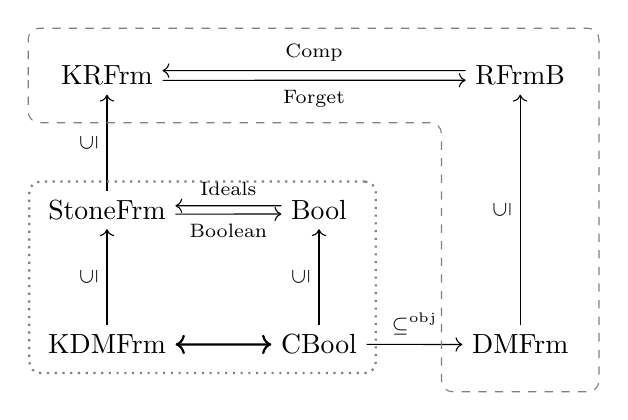
\begin{tikzpicture}[descr/.style={fill=white,inner sep=2.5pt}]
    \tikzset{
      mymx/.style={
        matrix of nodes,
        % nodes=block,
        row sep=3.5em,
        column sep=3.5em,
      },
      lbl/.style={
        % above,
        below,
        auto,
        % pos=0.15,
        % sloped, % make the text follow the path
        %execute at begin node={$}, % begin math mode, for the minus signs etc.
        %execute at end node={$}, % end math mode
      }
    }
    \tikzstyle{bigbox} = [draw=gray, thick, rounded corners, rectangle]

    \pgfmathsetmacro{\H}{1.0}
    \pgfmathsetmacro{\W}{0.6}

    \matrix (m) [mymx]
        { KRFrm & & RFrmB \\
          StoneFrm & Bool & \\
          KDMFrm & CBool & DMFrm \\
        };
    \path[->,font=\scriptsize,every node/.style=lbl]
        (m-2-1)     edge node {\InclUp} (m-1-1)
        (m-3-1)     edge node {\InclUp} (m-2-1)
        (m-3-3)     edge node {\InclUp} (m-1-3)
        (m-3-2)     edge node {\InclUp} (m-2-2)
        (m-3-2)     edge node {$ \subseteq^{\text{obj}}$} (m-3-3)

        % Stone duality
        (m-2-2) edge[transform canvas={yshift=1.5pt}]  node[swap] {Ideals}  (m-2-1)
        (m-2-1) edge[transform canvas={yshift=-1.5pt}] node[swap] {Boolean} (m-2-2)

        % Compact. Reflection
        (m-1-1.355) edge node[swap] {Forget} (m-1-3.185)
        (m-1-3.175) edge node[swap] {Comp} (m-1-1.5);

    \path[<->, thick]
        (m-3-1) edge node {} (m-3-2);


    \node[bigbox, dotted] [fit = (m-2-1) (m-3-2)] {};
    \draw[gray, rounded corners, dashed]
           ($(m-1-1) + (-\H,   0)$)
        -- ($(m-1-1) + (-\H, +\W)$)
        -- ($(m-1-3) + (+\H, +\W)$)
        -- ($(m-3-3) + (+\H, -\W)$)
        -- ($(m-3-3) + (-\H, -\W)$)
        -- ($(m-1-3) + (-\H, -\W)$)
        -- ($(m-1-1) + (-\H, -\W)$)
        -- ($(m-1-1) + (-\H,   0)$);
\end{tikzpicture}
\end{center}

\begin{diagram}[row sep=0.7cm]
    \StoneFrm
        \ar[yshift=0.2em]{r}{\scalebox{1.5}\Bc}
    & \Bool
        \ar[yshift=-0.2em]{l}{\scalebox{1.5}\J} \\
    \\
    \sigma\text{--}\categoryStyle{BDStoneFrm}
        \ar[yshift=0.2em]{r}{\scalebox{1.5}\Bc}
        \ar{uu}{\InclUp}
    & \sigma\text{--}\ComplBool
        \ar{uu}{\InclUp}
        \ar[yshift=-0.2em]{l}{\scalebox{1.5}\J} \\
    \DotsUp
        \ar{u}{\InclUp}
    & \DotsUp
        \ar{u}{\InclUp} \\
    \kappa\text{--}\categoryStyle{BDStoneFrm}
        \ar[yshift=0.2em]{r}{\scalebox{1.5}\Bc}
        \ar{u}{\InclUp}
    & \kappa\text{--}\ComplBool
        \ar{u}{\InclUp}
        \ar[yshift=-0.2em]{l}{\scalebox{1.5}\J} \\
    \DotsUp
        \ar{u}{\InclUp}
    & \DotsUp
        \ar{u}{\InclUp} \\
    \ExtrStoneFrm
        \ar[yshift=0.2em]{r}{\scalebox{1.5}{$\Bo\;\cong\;\Bc$}}
        \ar{u}{\InclUp}
    & \ComplBool
        \ar{u}{\InclUp}
        \ar[yshift=-0.2em]{l}{\scalebox{1.5}\J} \\
\end{diagram}

\section{Uniformity and metrizability}
\section{Non--metrizability of compactification}
\begin{lemma}
    For $L$ normal frame: $\sigma(x)\vee\sigma(x) = \sigma(x\vee y)$.
\end{lemma}

\chapter{Conclusion}
TODO or Further work?


\bibliographystyle{plain}
\bibliography{refs.bib}

\clearpage
% \addcontentsline{toc}{chapter}{Index}
\printindex
\end{document}
